\documentclass[12pt]{report}

\usepackage[a4paper,
            bindingoffset=0.5cm,
            left=2.5cm,
            right=2.5cm,
            top=5cm,
            bottom=5cm]{geometry}

\usepackage[english]{babel}
\usepackage{amsfonts}
\usepackage{titlesec}
\usepackage{hyperref}
\usepackage{listings}
\usepackage{xcolor}
\usepackage{graphicx}
\graphicspath{ {./img/} }
\usepackage{subcaption}

\renewcommand{\chaptermark}[1]{\markboth{\thechapter. #1}{}}
\titleformat{\chapter}{\normalfont\huge\bfseries}{\thechapter}{0.35cm}{}

\renewcommand{\lstlistingname}{Source code}
\lstset{language=Python, numbers=left, numbersep=10pt, backgroundcolor=\color{lightgray}}

\usepackage{caption}
\DeclareCaptionFont{white}{\color{white}}
\DeclareCaptionFormat{listing}{\colorbox{darkgray}{\parbox{\textwidth}{#1#2#3}}}
\captionsetup[lstlisting]{format=listing,labelfont={white, bf},textfont=white}

\lstdefinestyle{mystyle}
{
     frame=b,         
     belowcaptionskip=-1pt,
     xleftmargin=25pt,
     framexleftmargin=25pt,
     framexrightmargin=5pt,
     framextopmargin=5pt,
     framexbottommargin=5pt,
     framesep=0pt,
     rulesep=0pt,
     breaklines=true,
     showstringspaces=false
}

\lstset{literate=%
  {Ö}{{\"O}}1
  {Ä}{{\"A}}1
  {Ü}{{\"U}}1
  {ß}{{\ss}}1
  {ü}{{\"u}}1
  {ä}{{\"a}}1
  {ö}{{\"o}}1
} 

\begin{document}
\pagenumbering{gobble}
\vspace*{2cm}
\begin{center}
\textbf{\Huge Ray-tracing based renderer from scratch}
\end{center}
\vspace*{1cm}
\begin{figure}[h!]
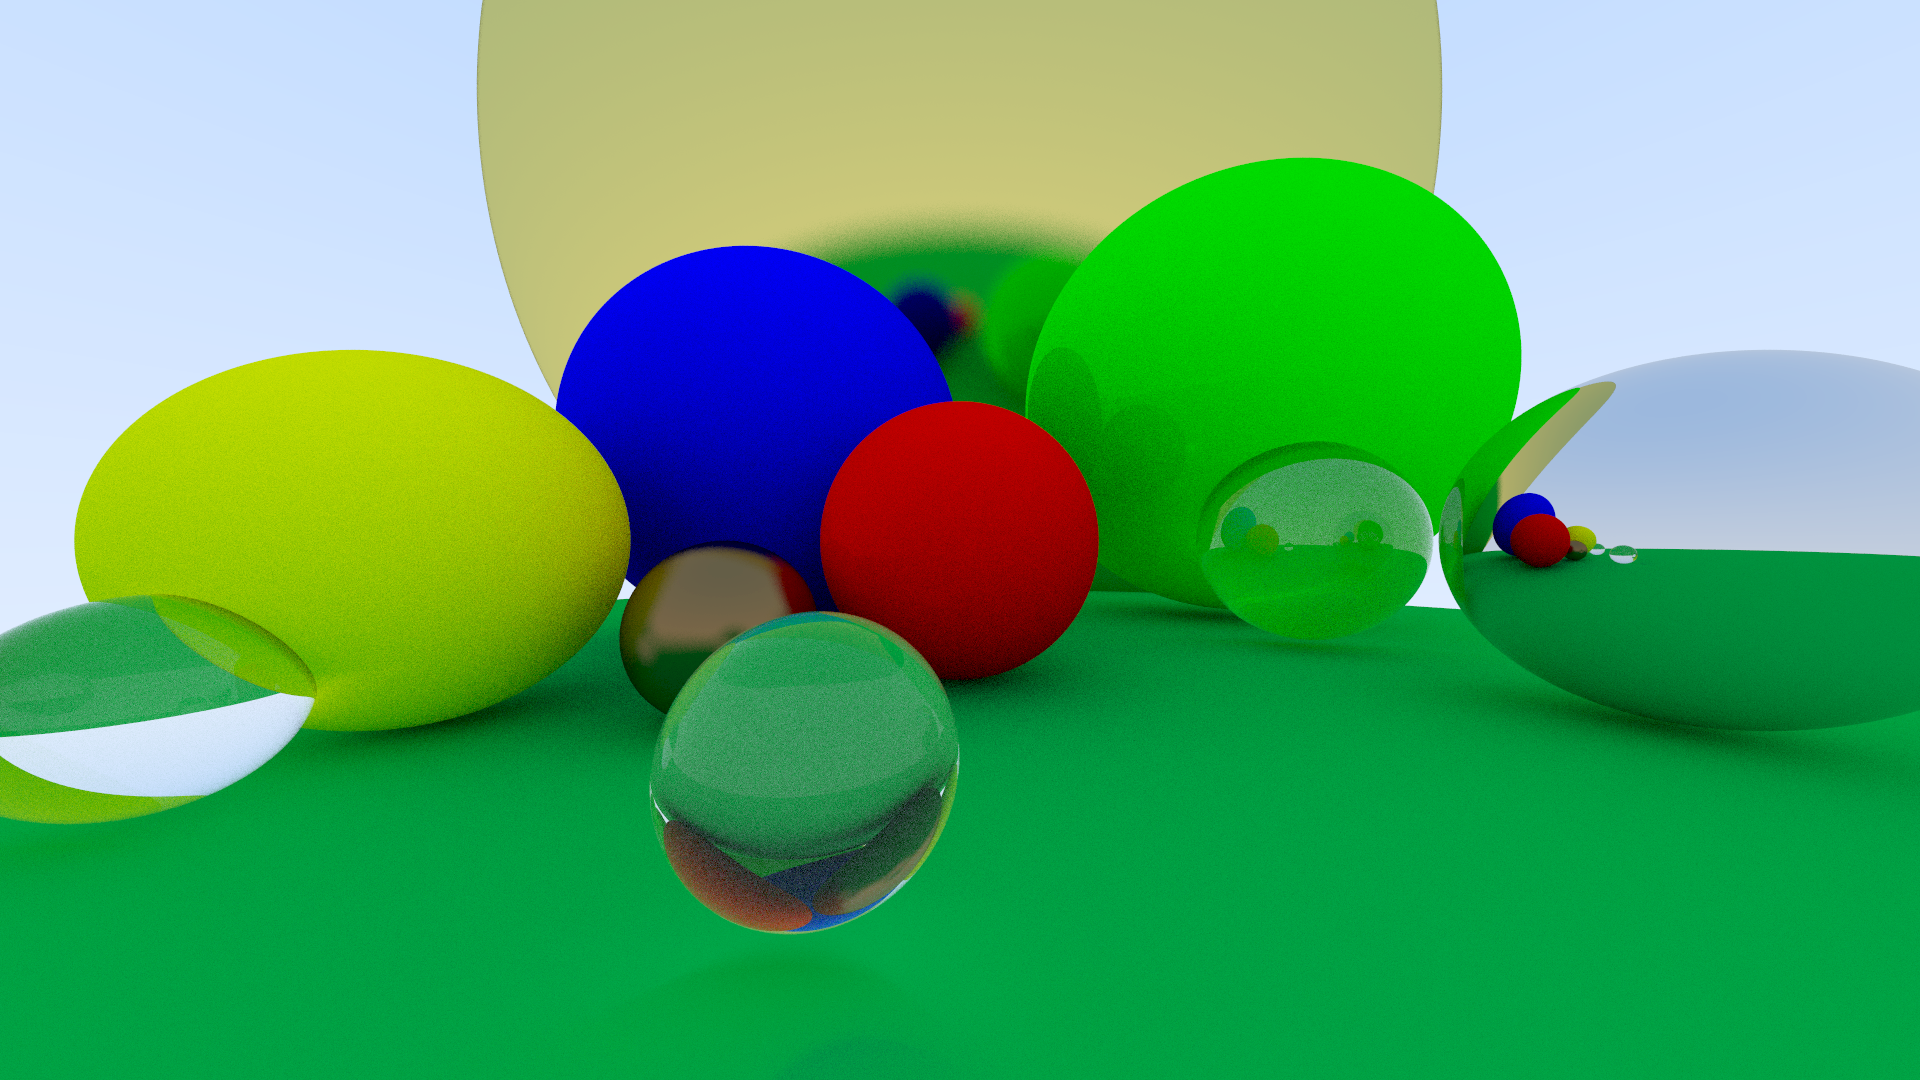
\includegraphics[width=\textwidth]{title}
\end{figure}
\begin{center}
{\Large Timo Salisch}
\end{center}
\clearpage

\tableofcontents

\newpage
\chapter{Rendering loop}
\label{chp:step1}
\pagenumbering{arabic}
The rendering process consists of two loops. One outer loop which iterates through the rows of the image and the inner loop iterating through the columns of the image. This way, every pixel will be visited once and the color of the pixel can be calculated. In this basic version of the rendering loop the color of every pixel will be set to (128, 64, 255). The resulting image can be seen in figure \ref{fig:step1}.
\begin{figure}[h!]

\includegraphics[width=\textwidth]{step1}
\centering
\caption{Result after running simple rendering loop}
\label{fig:step1}
\end{figure} \\
To store the already rendered information about the image, an \textit{Image} class is implemented. An instance of this class represents one image and saves the color information of every pixel using a two dimensional list. The color is represented as an instance of the \textit{Vector} class. This \textit{Vector} class saves three floating point values and offers simple arithmetic operations of (three-dimensional) vectors. These three values can either be interpreted as the world coordinates x, y and z or as the color properties red, green and blue. To change the color value of a specific pixel of the image, the \textit{Image} class provides an \textit{update} method to do so. In order for the image to be viewed, it has to be saved. The image is saved in the ''PPM'' format. This is done by the \textit{save\_image} method which expects a path and then saves the image to that path using the ''PPM'' format. For the file to be readable as ''PPM'', the first three lines have to include: ''P3'', image width and height, max color value. The actual pixel information are added by the loop iterating through the pixels. It is import to iterate through the rows beginning with the top row, otherwise the image is flipped. The saving process can be seen in source code \ref{lst:saving}.
\begin{lstlisting}[caption={Saving an image}, label=lst:saving, style=mystyle]
def save_image(self, path: str):
    image_str = f'P3\n{self.width} {self.height}\n255'
  
    for j in range(self.height)[::-1]:
        for i in range(self.width):
            red, green, blue = self.matrix[i][j].to_tuple()
            image_str = image_str + f"\n{int(red)} {int(green)} {int(blue)}"

    with open(path, mode='w+') as f:
        f.write(image_str)
\end{lstlisting}

\chapter{Camera}
The project is extended by a \textit{Ray} and \textit{Camera} class. A ray can be used to find all objects that need to be projected onto one pixel and thus finding the color of a pixel. Every ray has an origin and a direction, with both being instances of the \textit{Vector} class. It is possible to get the position of a ray through its method \textit{position}. The camera represents the observer of the scene and has properties such as position and information about the image. The rendering loop from chapter \ref{chp:step1} is moved into the camera class. It uses the cameras properties to find the color for every pixel. This is done by sending a ray from the camera to every pixel and finding the color of this ray. Because there are no objects in the scene yet, the color of a ray is the color of the background at that position as shown in source code \ref{lst:step2}.
\begin{lstlisting}[caption={Color of ray}, label=lst:step2, style=mystyle]
def get_color(ray: Ray):
    unit_direction = ray.direction.normalize()
    t = 0.5 * (unit_direction.y + 1)
    ray_color = Vector(255, 255, 255) * (1 - t) + Vector(127.5, 178.5, 255) * t
    return ray_color
\end{lstlisting}
This results in an image which goes from light blue at the top to a white color at the bottom, as can be seen in figure \ref{fig:step2}.
\begin{figure}[h!]

\includegraphics[width=\textwidth]{step2}
\centering
\caption{Rendering with camera and colored background}
\label{fig:step2}
\end{figure}

\chapter{Objects: shape}
After adding a camera to the scene, the next logical step is to add objects. The chosen object to start with are spheres. For this a class \textit{Sphere} is implemented, which takes a vector as origin, a radius and a color vector. A \textit{Sphere} instance can return if a given ray hits it and if so, can calculate the intersection point of the ray and itself and its normal vector at that point. The normal vector is chosen to always point outwards of the sphere. If a ray hits a sphere, the ray adopts the color of the sphere. To better organize the handling of the sphere objects, a \textit{Scene} class is used. This class represents the scene and holds the camera and all objects in this scene. The objects are stored in an instance of the \textit{World} class. This class is basically an abstracted list with the benefit, that it provides a \textit{hit} method. Like the equivalent method of the \textit{Sphere} class, it determines if the ray hits an object. But this method checks all spheres and returns the information about the sphere, that gets hit by the ray first. This solves the visibility problem of multiple spheres being stacked behind each other. It also simplifies the rendering loop to not having to iterate through all spheres, because this is done internally by this method. To keep the interface simple, the \textit{Scene} class also offers a \textit{render} method which just forwards to the equivalent method of the camera. This way, all required actions can be performed using a \textit{Scene} instance which, after rendering, returns an \textit{Image} instance that can be used as needed. To change the scene after creation, it provides a function to add spheres to it. This class structure simplifies the whole process from creating to rendering and saving the image to:
\begin{itemize}
\item Creating a \textit{Camera} instance with preferred properties
\item Creating a \textit{Scene} object giving the camera instance as a parameter
\item Creating and adding as many \textit{Sphere} instances to the scene object as wanted
\item Using \textit{render} function of scene
\item Saving resulted \textit{Image} object to any path
\end{itemize}
Using this procedure, images can be created that contain multiple spheres. Every sphere can have a different color, position and size. If at a position in the image there is no sphere, the background color introduces in the previous chapter is kept. At this point the created rendered has solved the visibility problem, even though in a pretty simple setting. An example of an image created by this renderer is displayed in figure \ref{fig:step3}.
\begin{figure}[h!]
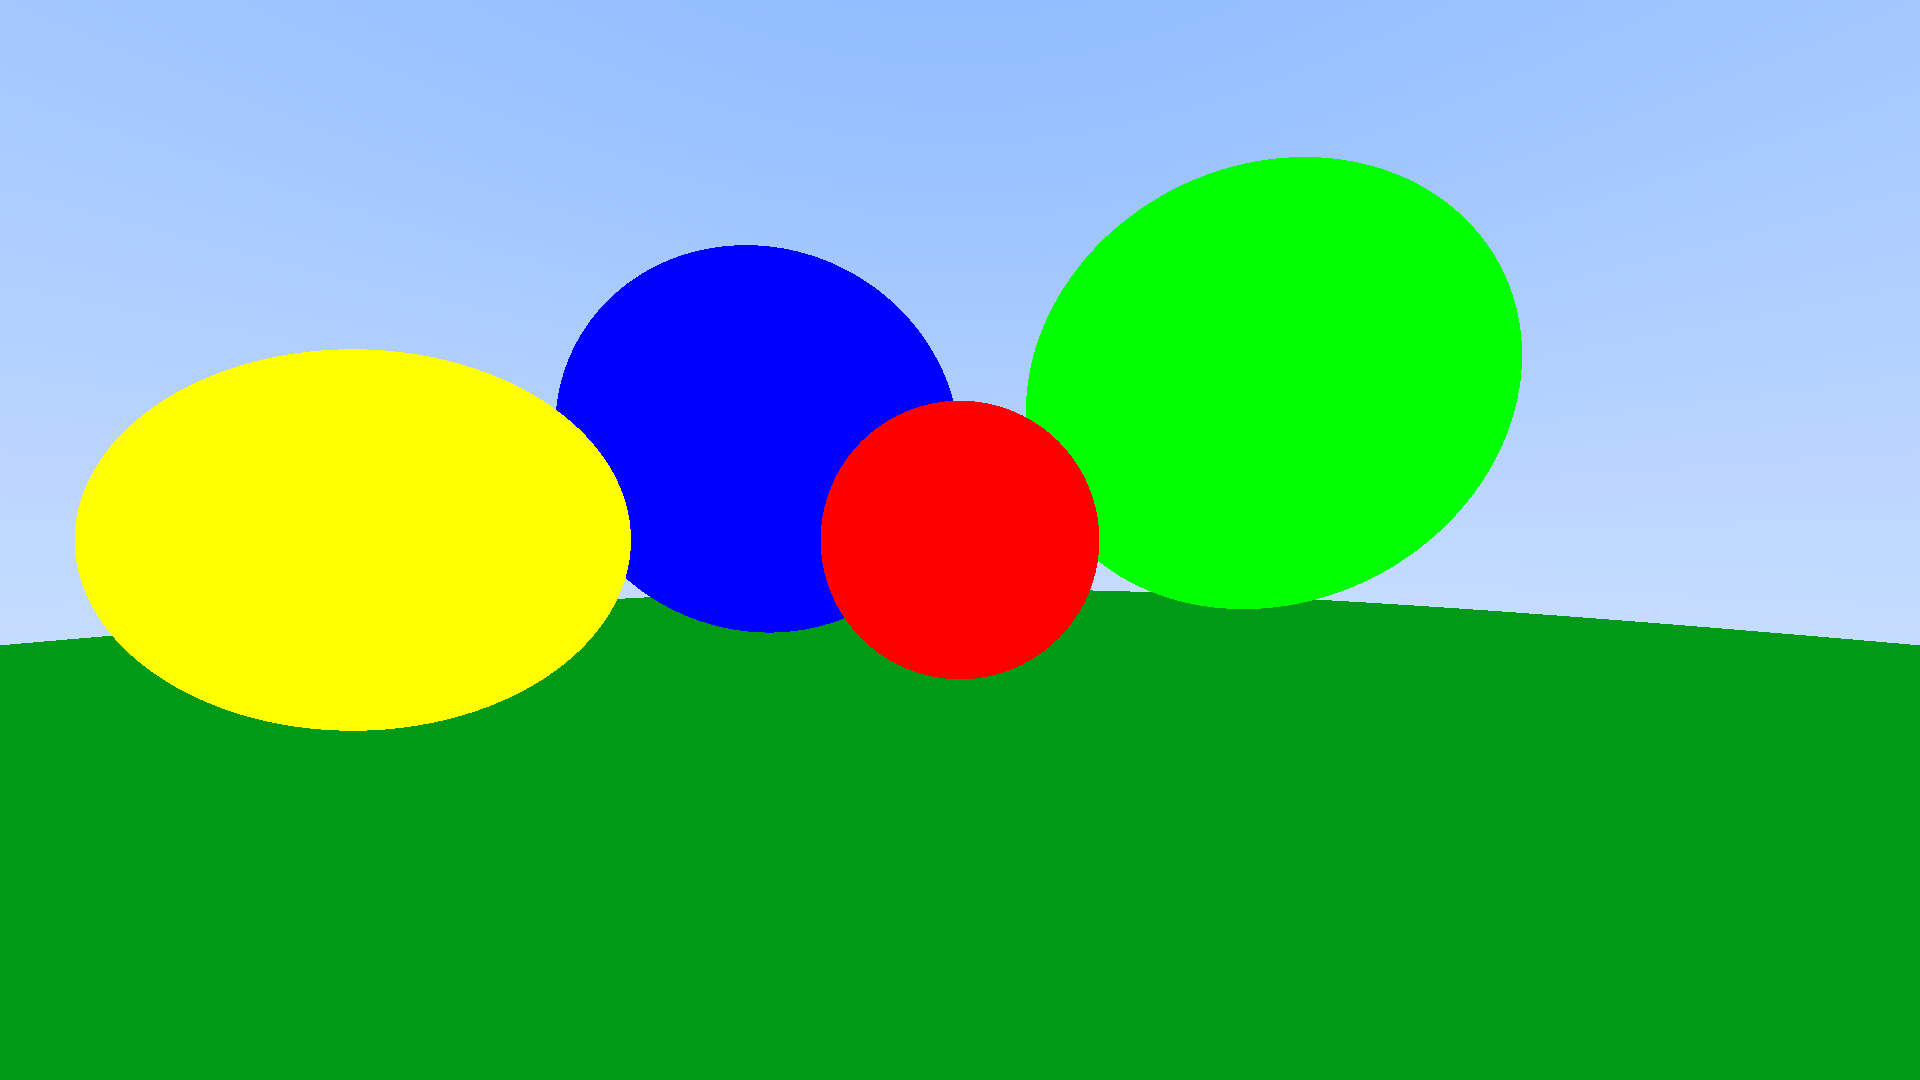
\includegraphics[width=\textwidth]{step3}
\centering
\caption{Image created by simple renderer}
\label{fig:step3}
\end{figure}

\chapter{Enhancing camera and rendering loop}
On the rendered images the spheres seem round, but this is not the actually the case. They only look round because of the ''high'' quality and thus the pixels being pretty small. By zooming into the image at the border of a sphere this can be seen more clearly (figure \ref{fig:aliasing}).
\begin{figure}[h!]

\includegraphics[width=\textwidth]{aliasing}
\centering
\caption{Zoomed in sphere border}
\label{fig:aliasing}
\end{figure} \\
The reason for this is, that only one ray is sent through each pixel at the left end of the pixel. With spheres being round in reality but monitors only being able to display things using pixels, this is no unexpected behavior. But if pixels are bigger -- either because of a lower resolution or because the images are shown on a bigger screen -- this can make the image look unnatural and wrong. One way of improving the border would be using colors in between the two colors (here red and green). This would make the edge less harsh and thus the sphere looks more round. To keep the correct shape of the objects and not adding any visual bumps to it, the color has to be mixed of the two colors keeping the ratio of the objects in this pixel into account. To not having to calculate the ratio for every pixel, which is computational expensive, multiple rays are sent through each pixel at random positions of the pixel. The average color of these rays can then be used as the color of the pixel. The more rays are used per pixel, the closer will the average color be to the true color.
\begin{figure}[h!]
\centering
\begin{subfigure}[h!]{0.475\textwidth}
\centering

\includegraphics[width=\textwidth]{step4_2rays}
\caption{2 rays per pixel}
\end{subfigure}
\hfill
\begin{subfigure}[h!]{0.475\textwidth}
\centering

\includegraphics[width=\textwidth]{step4_4rays}
\caption{4 rays per pixel}
\end{subfigure}
\vskip\baselineskip
\begin{subfigure}[h!]{0.475\textwidth}
\centering

\includegraphics[width=\textwidth]{step4_8rays}
\caption{8 rays per pixel}
\end{subfigure}
\hfill
\begin{subfigure}[h!]{0.475\textwidth}
\centering

\includegraphics[width=\textwidth]{step4_16rays}
\caption{16 rays per pixel}
\end{subfigure}
\caption{Zoomed in sphere border with a different number of rays per pixel}
\label{fig:step4}
\end{figure} \\
From figure \ref{fig:step4} can be seen, that the more rays are used per pixel the more different color shades are used at the sphere's border. In comparison to only one ray (figure \ref{fig:aliasing}), it is visible that the sphere's edge becomes much smoother the more rays are used.

\chapter{Objects material: diffuse}
jhfjgjkfgjfghjjfg

\chapter{Objects material: specular}
jhfjgjkfgjfghjjfg

\chapter{Objects material: specular transmission}
jhfjgjkfgjfghjjfg

\chapter{Lights}
jhfjgjkfgjfghjjfg

\chapter{Positioning and orienting camera}
jhfjgjkfgjfghjjfg

\chapter{Animation}
jhfjgjkfgjfghjjfg

\chapter{Render parallelization}
jhfjgjkfgjfghjjfg

\chapter{Config files}
jhfjgjkfgjfghjjfg
\end{document}